\documentclass[times, utf8, seminar]{fit}

%\batchmode
%\usepackage{booktabs}
\usepackage{listings}
\usepackage{longtable}
\usepackage{xcolor}
\usepackage{float}
\usepackage{enumitem}
\usepackage{hyperref}
\usepackage{enumerate}
\usepackage{graphicx}
\usepackage{etoolbox}

\begin{document}

\title{Projekat: Unapređenje informacionog sistema na primjeru jedne kompanije}

\author{Ernad Husremović}
\brindex{DL 2792}
\verzija {1.0.0}

\mentor{prof.dr Murat Prašo}

\maketitle

\tableofcontents

\listoftables
\listoffigures

% abstract begin
\begin{sazetak}


Sažetak na bosanskom jeziku.

\kljucnerijeci{bosanska rijec 1, bosanska rijec 2}
\end{sazetak}

\engtitle{Naslov na engleskom jeziku}
\begin{abstract}
Abstract na engleskom jeziku.

\keywords{key1, key2, key3}
\end{abstract}

% abstract end

\chapter{Uvod}

\section{Legalizacija - bezpovratne promjene na IT tržištu BiH}

Akcije državnih inspekcijskih organa na suzbijanju nelegalnog softvera (nadalje legalizacija) sa početkom 2012 godine označila je početak krupnih promjena na tržištu informatičkih \engl{information technology, nadalje IT} rješenja u Bosni i Hercegovini. 
Većina poslovnih subjekata koja se u proteklim godinama opremila "jeftinim" nelegalnim softverom \engl{software} našla se u nezavidnoj situaciji.
Usljed visokih troškovima legalizacije "Microsoft" softvera\footnote{familija "Microsoft Windows" OS-ova, uz svuda prisutni ali i redovno nelegalno instalirani "Microsoft Office" uredski paket}, pojavila se potražnja za softverom drugih proizvođača.  

\section{OSS software}

Preduzeće "bring.out"\footnote{\url{http://www.bring.out.ba/}} je dugi niz godina orjentisano na ponudu sistema baziranih na software-u otvorenog koda \engl{open source software, nadalje OSS}.

Potražnja za Linux/Ubuntu serverskim rješenjima \footnote{\url{http://linux.com}, \url{http://ubuntu.com}}) je postojala i prije legalizacije. Međutim, tek nakon legalizacije pojavila se potražnja za cjelovitim informatičkim IT rješenjima baziranim na OSS-u:
\begin{itemize}
  \item server operativni sistem (nadalje OS)
  \item desktop operativni sistem
  \item aplikativni softver
  \begin{itemize}
    \item opći software za uredske potrebe
    \item poslovni - softver \engl{Enterprise Resource Planning, nadalje ERP}
  \end{itemize}
\end{itemize}

\subsection{Ubuntu Linux}
"Ubuntu" Linux distribucija radi svoje jednostavnosti i kvaliteta postao popularan desktop OS.

Za razliku od "Windows" operativnih sistema, "Ubuntu" desktop sistem sadrži kompletan set aplikacija za svakodnevne potrebe:
\begin{itemize}
  \item LibreOffice uredski paket za pravljenje tekstualnih i tabelarnih dokumenata, prezentacija i crteža\footnote{Pandam "Microsoft office" setu aplikacija. Otvara većinu "Microsoft office" dokumenata }
  \item "Inkscape" za vektorsku grafiku
  \item "GIMP" za bitmapiranu graviku
  \item "Evince" preglednik PDF dokumenata
  \item "Firefox", "Chromium" internet pretraživači
\end{itemize}  
 
Ovim se lista dostupnih aplikacija ne završava. Međutim, i to je dovoljno u poređenju sa "Windows" OS-om koji se isporučuje bez ikakvih aplikacija.

Unutar ovog projekta će se OSS koristiti za gradnju jednog kompletnog informacionog sistema.

\subection{F18 knowhowERP software}
Pored standardnih komponentni "Ubuntu" OS-a, za ERP softver će se koristiti "F18" knowhowERP software.

F18\footnote{\url{http://redmine.bring.out.ba/projects/f18}} je multiplatformski OSS softver, proizvod firme "bring.out".  

\subsection{Cjelovito OSS IT rješenje}
Na osnovu do sada rečenog, bosanskom klijentu je moguće ponuditi cjelovito OSS IT rješenje.  

Ovaj projekat će obuhvatiti instalaciju jednog takvog sistema kod klijenta.

Komparativnom analizom utvrdićemo toškove sličnog sistema baziranog na zatvorenim tehnologijama:
\begin{enumerate}[(a)]
  \item sa uključenim troškovima legalizacije postojećeg nelegalnog "Windows" OS softvera bez zamjene postojećeg ERP aplikativnog softvera
  \item sa kompletnom zamjenom kako sistemskog, tako i aplikativnog ERP softvera.  
\end{enumerate}

\section{Profil korisnika projekta}
Korisnik je mala kompanija koja se bavi trgovinom. Sa stanovišta IT-a kompanija se sastoji od:
\begin{itemize}
  \item maloprodajna mreža od 5 prodavnica
  \item centrala kompanije sa knjigovodstvom, 4 radne stanice
  \item 1 server baze podataka 
\end{itemize}

\chapter{Analiza}

\section{Analiza problema}

Povod klijentu za traženje novog rješenja je nedavna akcija legalizacije. 

Međutim, analiza je pokazala da su glavni problemi leže u činjenici da postojeći poslovni IS ne obezbjeđuje sve potrebne podatke. Već nakon prvog sastanka sa klijentom utvrđeni su sljedeći problemi, prikazani piramidmo problema:

\begin{figure}[H]
\centering
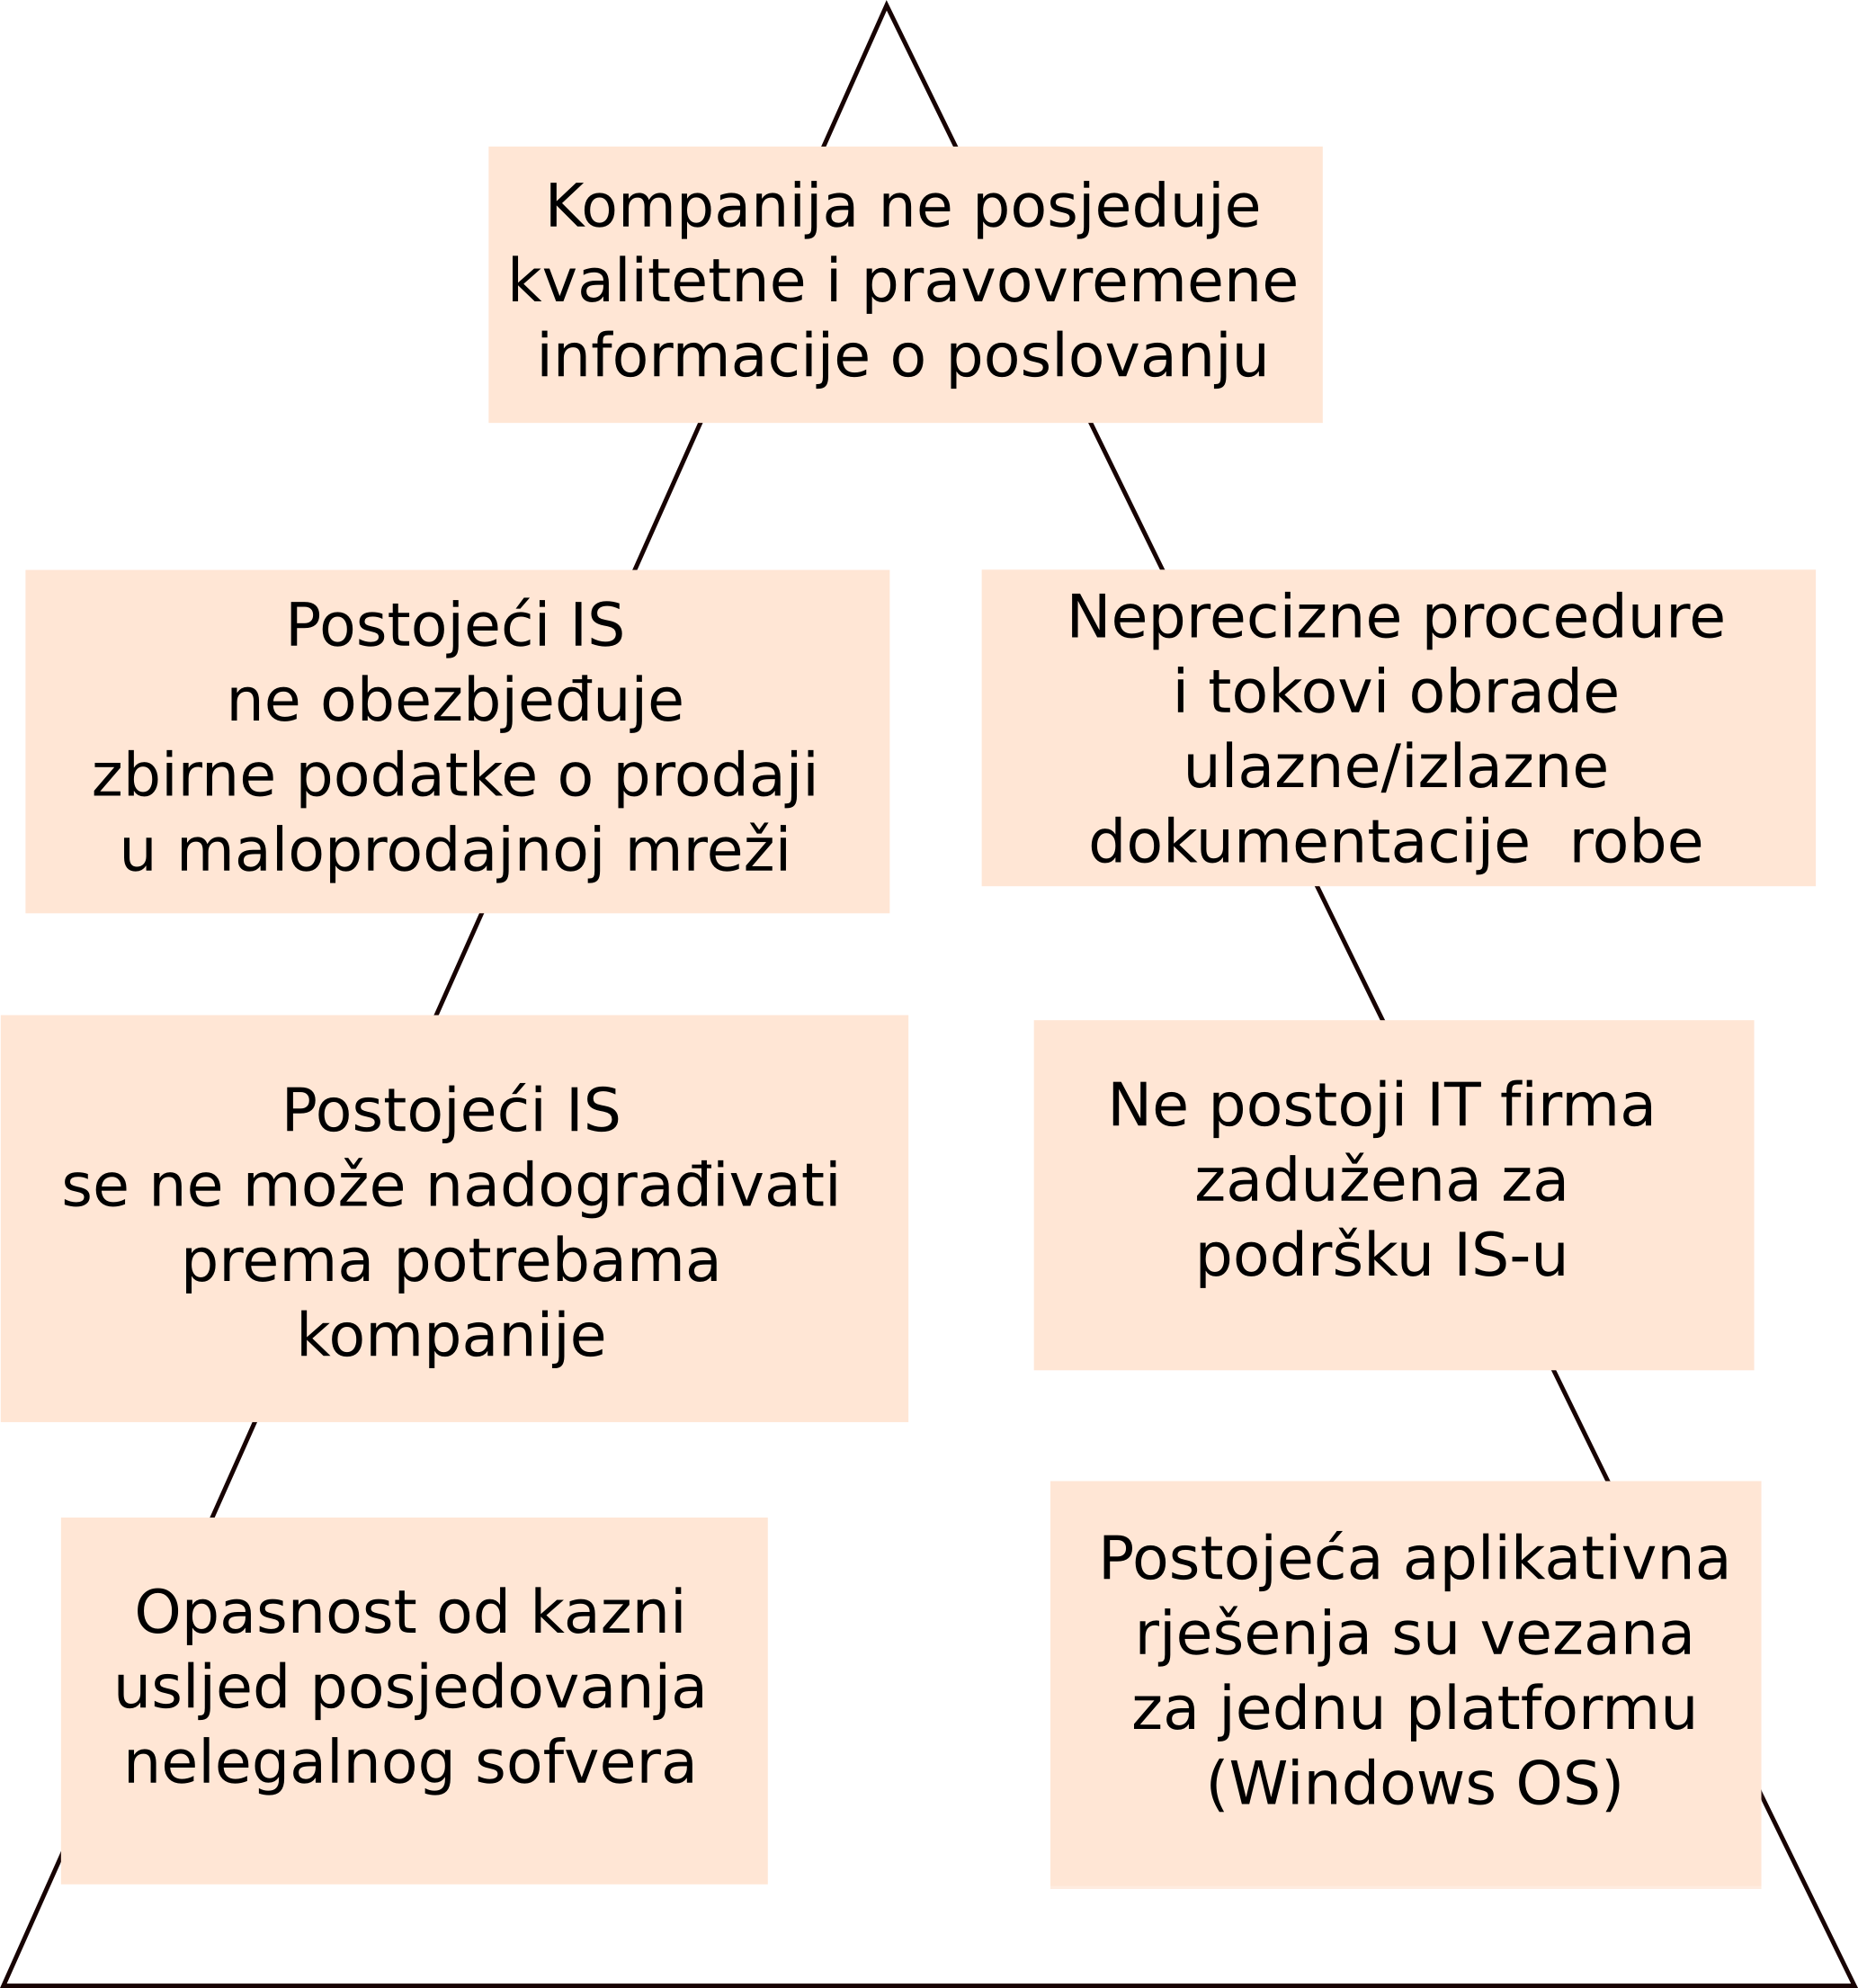
\includegraphics[width=12cm]{img/piramida_problema.png}
\caption{Piramida problema}
%\caption{bla bla (\cite{web:eric})}
\end{figure}

Piramida na vrhu prikazuje opće probleme da bi se idući ka dnu ti problemi konkretizirali.  

\section{Analiza cilja}
Analizom problema prezentovanih piramidom problema brzo dolazimo do strateškog cilja ovog projekta:
%\patchcmd{\quote}{\rightmargin}{\leftmargin 6em \rightmargin}{}{}
\begin{quote}
\em Uvođenjem novog IS-a poboljšati pravovremenost i kvalitet tekućih informacija o poslovanju.} 
\end{quote}
Analogno ranijem grafičkom prikazu problema, putem piramide ciljeva od dna ka vrhu prezentujemo ciljeve čijom realizacijom postižemo strateški cilj:

\begin{figure}[H]
\centering
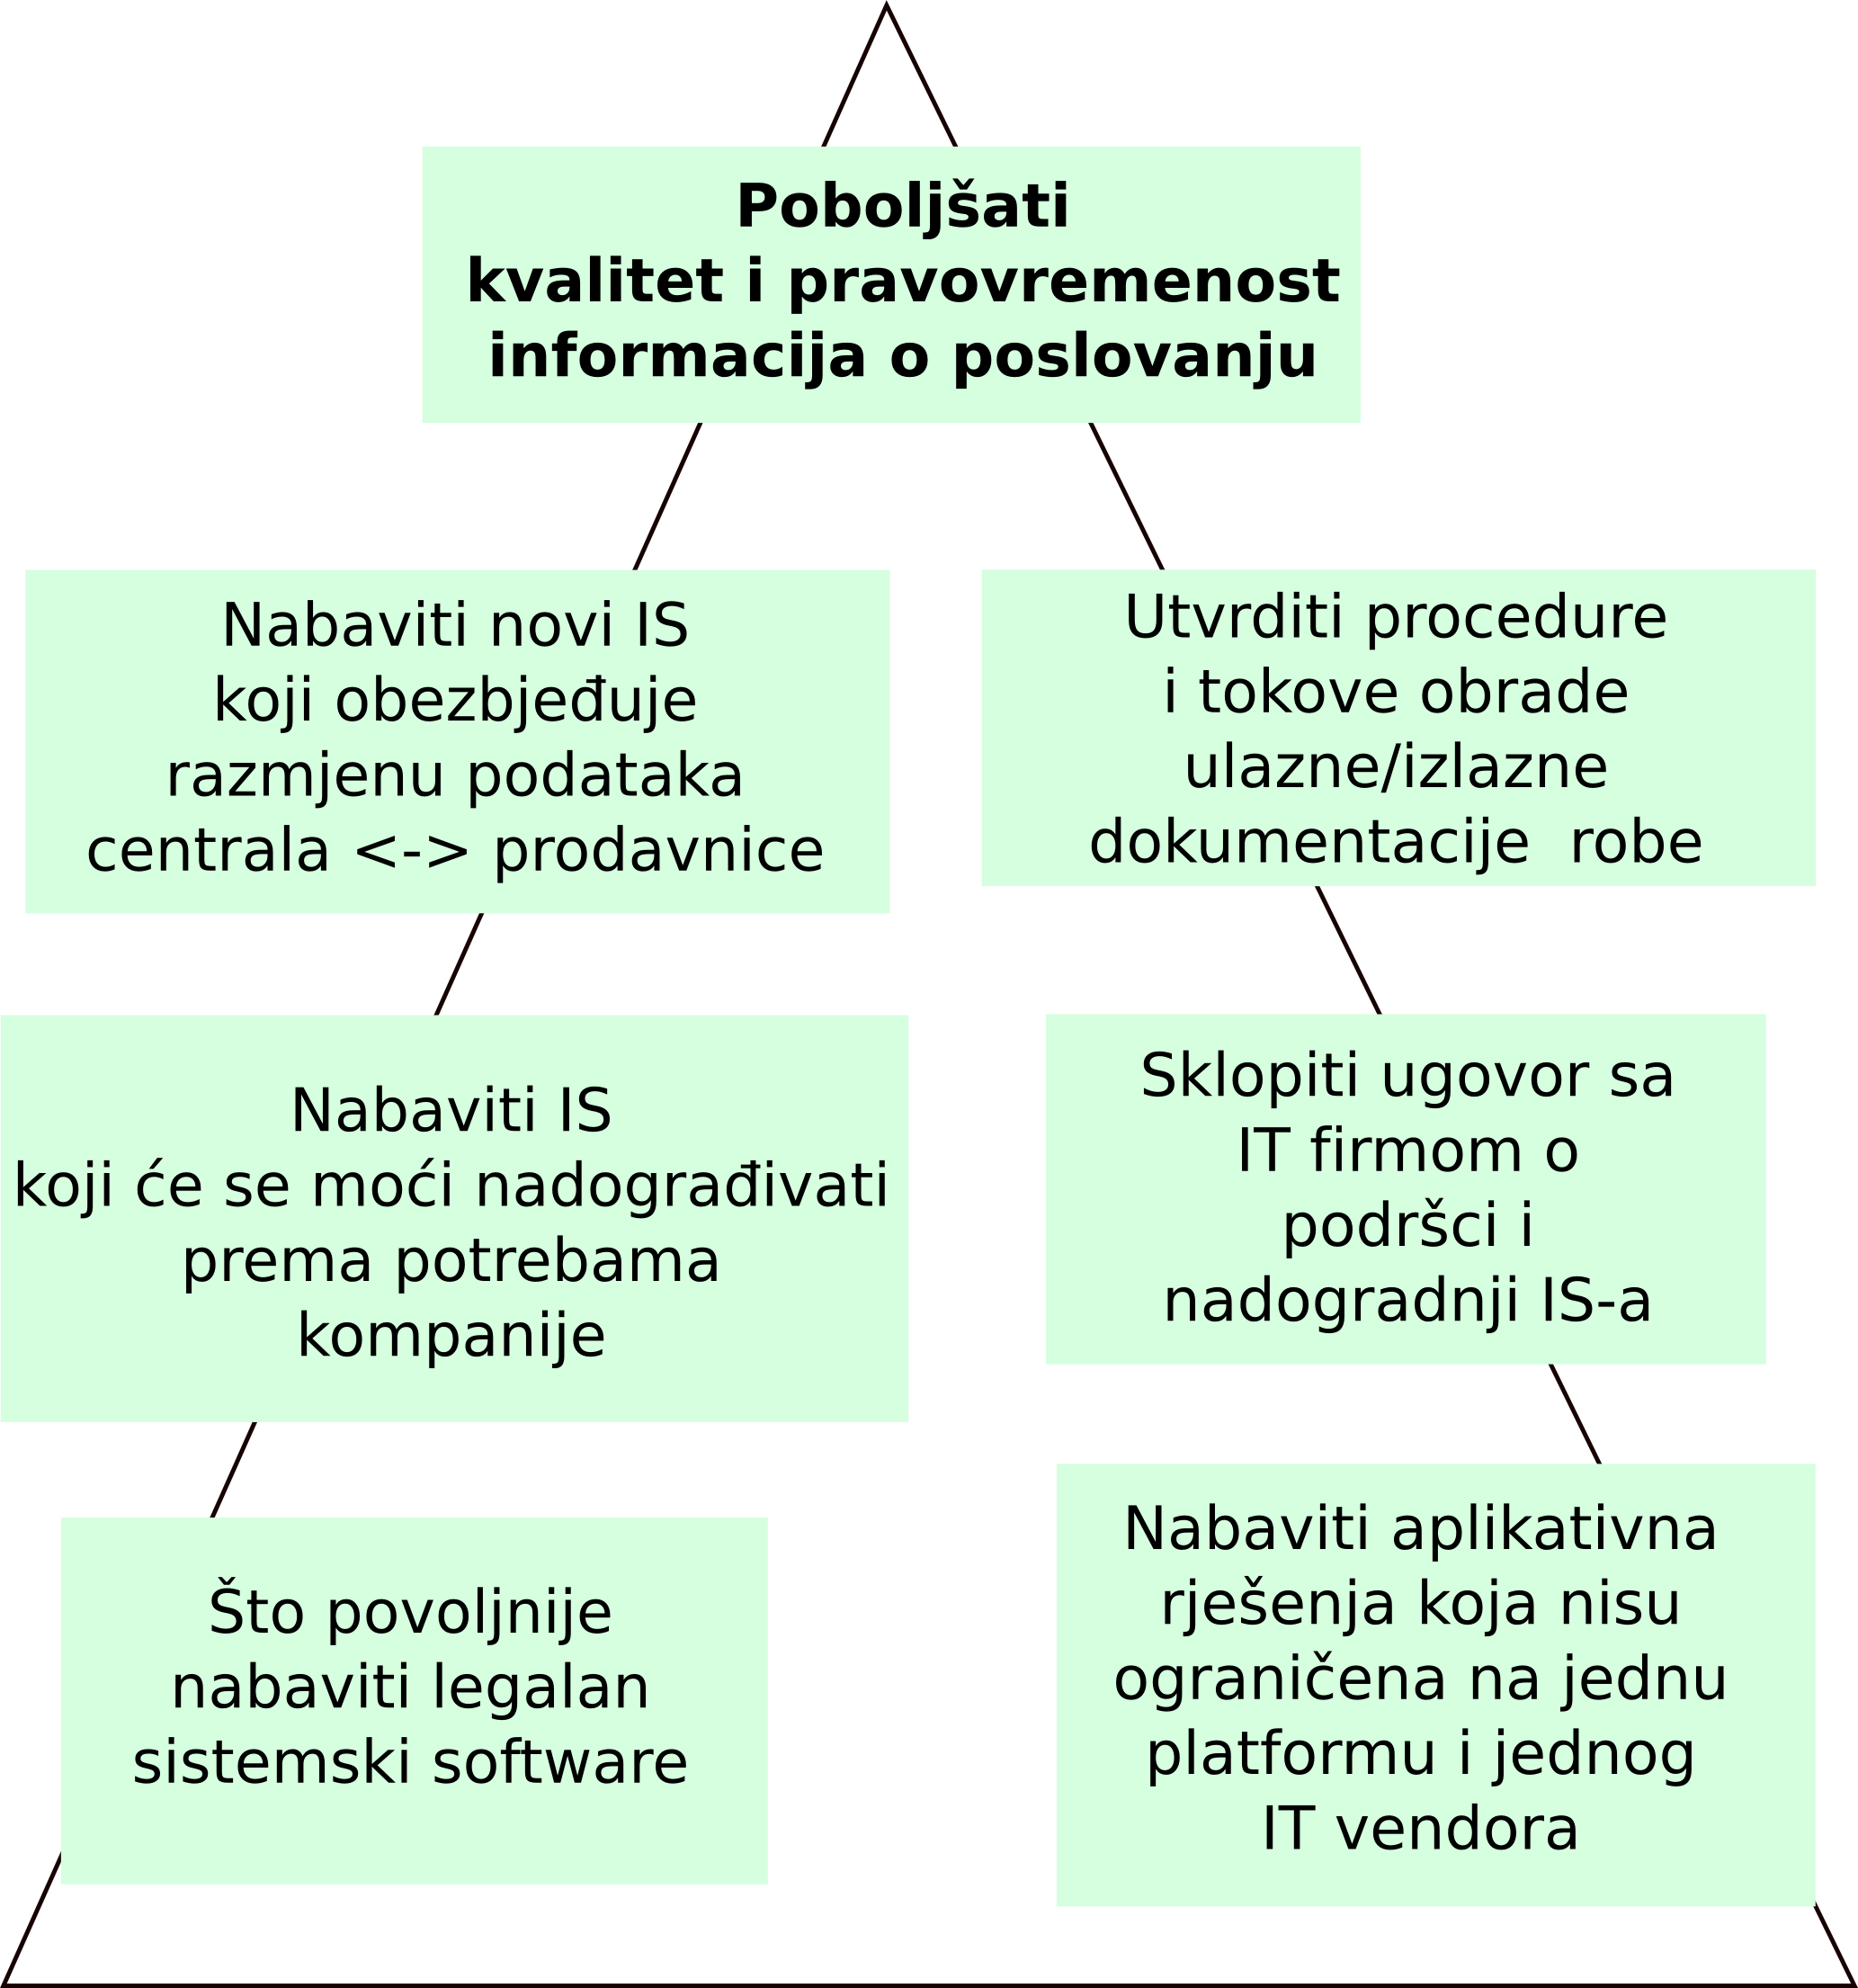
\includegraphics[width=12cm]{img/piramida_cilja.png}
\caption{Piramida cilja}
\end{figure}

\section{Logički okvir projekta}
Na kraju analize dolazimo do ključnih odrednica projekta:
\begin{table}[h]
%\centering
\resizebox{15cm}{!} {
\begin{tabular}{ | r | l | }
\hline
Svrha projekta: & Unapređenje poslovanja kompanije obezbjeđenjem kvalitetnijih informacija o poslovanju \\ \hline
Cilj: & Uvođenje novog informacionog sistema \\ \hline
Ulazi projekta: & Postojeći informacioni sistem, postojeća organizacija poslovanja \\ \hline
Izlazi projekta: & Unapređeni informacioni sistem, unapređena organizacija poslovanja \\ \hline
\end{tabular}
}

\caption{Logički okvir projekta}
\end{table}


\label{tab:myfirsttable}
\label{labela_oznaka}

\begin{description}
  \item [item 1]  objasni item 1
  \item [item 2] objasni item 2
\end{description}
 

Citacija \cite[str.~391]{pentaho32}.

\begin{itemize}
   \item vako 
   \item nako
\end{itemize}

Referenca na sekciju sekcija1 (vidi \ref{sect:sekcija1}).
 
\section{Sekcija 1 sa slikom}
\label{sect:sekcija1}

\begin{figure}[H]
\centering
\includegraphics[width=15cm]{img/vako_nako.pdf}
\caption{vako nako caption}
\end{figure}


\section{Zaključak}

\bibliography{literatura}
\bibliographystyle{fit}

\appendix

\chapter{dodatak 1}
\label{chap:dodatak1}

\chapter{Korišteni softver}

Softver korišten za realizaciju ovog dokumenta:
\begin{enumerate}
  \item Mac OS X 10.6.8
  \item Ubuntu Linux 12.04 Unity, 64bit
  \item mvim, vim tekst editor ver 7.3
  \item MacTex - pdfTeX 3.1415926-2.3-1.40.12 (TeX Live 2011)
  \item Windows XP Proffesional on VirtualBox 4.1.16 MacOSX 
  \item Microsoft Project 2010, trial, ProductID 02252-552-2789414-37542
  \item LibreOffice 3.5.4 ?
  \item Inkscape ?
\end{enumerate}

\begin{itemize}

\chapter{Bilješke}
\label{chap:biljeske}

\begin{enumerate}
  \item jedan
  \item dva: \url{http://redmine.bring.out.ba/issues/26711}
\end{enumerate}

\end{document}
